%me=0 student solutions (ps file), me=1 - my solutions (sol file), me=2 - assignment (hw file)
\def\me{0}
\def\num{6}  %homework number
\def\due{Wednesday, March 25}  %due date
\def\course{CSCI-UA.0310-004/005 Basic Algorithms} %course name, changed only once
\def\name{Jason Yao}   %student changes (instructor keeps!)
%
\iffalse
INSTRUCTIONS: replace # by the homework number.
(if this is not ps#.tex, use the right file name)

  Clip out the ********* INSERT HERE ********* bits below and insert
appropriate TeX code.  Once you are done with your file, run

  ``latex ps#.tex''

from a UNIX prompt.  If your LaTeX code is clean, the latex will exit
back to a prompt.  To see intermediate results, type

  ``xdvi ps#.dvi'' (from UNIX prompt)
  ``yap ps#.dvi'' (if using MikTex in Windows)

after compilation. Once you are done, run

  ``dvips ps#.dvi''

which should print your file to the nearest printer.  There will be
residual files called ps#.log, ps#.aux, and ps#.dvi.  All these can be
deleted, but do not delete ps1.tex. To generate postscript file ps#.ps,
run

  ``dvips -o ps#.ps ps#.dvi''

I assume you know how to print .ps files (``lpr -Pprinter ps#.ps'')
\fi
%
\documentclass[11pt]{article}
\usepackage{amsfonts}
\usepackage{listings}
\usepackage{latexsym}

\usepackage{tikz}

\setlength{\oddsidemargin}{.0in}
\setlength{\evensidemargin}{.0in}
\setlength{\textwidth}{6.5in}
\setlength{\topmargin}{-0.4in}
\setlength{\textheight}{8.5in}

\newcommand{\handout}[5]{
   \renewcommand{\thepage}{#1, Page \arabic{page}}
   \noindent
   \begin{center}
   \framebox{
      \vbox{
    \hbox to 5.78in { {\bf \course} \hfill #2 }
       \vspace{4mm}
       \hbox to 5.78in { {\Large \hfill #5  \hfill} }
       \vspace{2mm}
       \hbox to 5.78in { {\it #3 \hfill #4} }
      }
   }
   \end{center}
   \vspace*{4mm}
}

\newcounter{pppp}
\newcommand{\prob}{\arabic{pppp}}  %problem number
\newcommand{\increase}{\addtocounter{pppp}{1}}  %problem number

%first argument desription, second number of points
\newcommand{\newproblem}[2]{
\ifnum\me=0
\ifnum\prob>0 \newpage \fi
\increase
\setcounter{page}{1}
\handout{\name, Homework \num, Problem \arabic{pppp}}{\today}{Name: \name}{Due:
\due}{Solutions to Problem \prob\ of Homework \num\ (#2)}
\else
\increase
\section*{Problem \num-\prob~(#1) \hfill {#2}}
\fi
}

%\newcommand{\newproblem}[2]{\increase
%\section*{Problem \num-\prob~(#1) \hfill {#2}}
%}

\def\squarebox#1{\hbox to #1{\hfill\vbox to #1{\vfill}}}
\def\qed{\hspace*{\fill}
        \vbox{\hrule\hbox{\vrule\squarebox{.667em}\vrule}\hrule}}
\newenvironment{solution}{\begin{trivlist}\item[]{\bf Solution:}}
                      {\qed \end{trivlist}}
\newenvironment{solsketch}{\begin{trivlist}\item[]{\bf Solution Sketch:}}
                      {\qed \end{trivlist}}
\newenvironment{code}{\begin{tabbing}
12345\=12345\=12345\=12345\=12345\=12345\=12345\=12345\= \kill }
{\end{tabbing}}

\newcommand{\eqref}[1]{Equation~(\ref{eq:#1})}

\newcommand{\hint}[1]{({\bf Hint}: {#1})}
%Put more macros here, as needed.
\newcommand{\room}{\medskip\ni}
\newcommand{\brak}[1]{\langle #1 \rangle}
\newcommand{\bit}[1]{\{0,1\}^{#1}}
\newcommand{\zo}{\{0,1\}}
\newcommand{\C}{{\cal C}}

\newcommand{\nin}{\not\in}
\newcommand{\set}[1]{\{#1\}}
\renewcommand{\ni}{\noindent}
\renewcommand{\gets}{\leftarrow}
\renewcommand{\to}{\rightarrow}
\newcommand{\assign}{:=}

\newcommand{\AND}{\wedge}
\newcommand{\OR}{\vee}

\newcommand{\For}{\mbox{\bf For }}
\newcommand{\To}{\mbox{\bf to }}
\newcommand{\Do}{\mbox{\bf Do }}
\newcommand{\If}{\mbox{\bf If }}
\newcommand{\Then}{\mbox{\bf Then }}
\newcommand{\Else}{\mbox{\bf Else }}
\newcommand{\While}{\mbox{\bf While }}
\newcommand{\Repeat}{\mbox{\bf Repeat }}
\newcommand{\Until}{\mbox{\bf Until }}
\newcommand{\Return}{\mbox{\bf Return }}
\newcommand{\Swap}{\mbox{\bf Swap }}

\begin{document}

\ifnum\me=0
%\handout{PS\num}{\today}{Name: Jason Yao}{Due:
%\due}{Solutions to Problem Set \num}
%
%I collaborated with *********** INSERT COLLABORATORS HERE (INDICATING
%SPECIFIC PROBLEMS) *************.
\fi
\ifnum\me=1
\handout{PS\num}{\today}{Name: Yevgeniy Dodis}{Due: \due}{Solution
{\em Sketches} to Problem Set \num}
\fi
\ifnum\me=2
\handout{PS\num}{\today}{Lecturer: Yevgeniy Dodis}{Due: \due}{Problem
Set \num}
\fi

\lstset{ %
breaklines=true,        % sets automatic line breaking
breakatwhitespace=false,    % sets if automatic breaks should only happen at whitespace
showtabs=false,                 % show tabs within strings adding particular underscores
frame=single,           % adds a frame around the code
tabsize=2,          % sets default tabsize to 2 spaces
escapechar=?,
}


\newproblem{Number of Predecessors}{8 points}

Assume you are given a binary search tree $T$ on $n$
elements.
Using a slight modification of the {\sc PostOrder-Tree-Walk}
procedure, argue (by writing the pseudocode!) that in time $\Theta(n)$ you can compute, for every
node $v$, the number of nodes (call it $v.less$) {\em in $v$'s
sub-tree} which are less than $v$.\\
\hint{In addition to $v.less$, also compute the total number of nodes
in $v$'s subtree.}

\begin{itemize}
\item[(a)] (5 points) Start with the simpler case when all the elements are distinct.


\ifnum\me<2
\begin{solution}

\begin{lstlisting}
int lessNodeFind(node v)
	return lessNodeFindRec(v.left, v.value)
end lessNodeFind

int lessNodeFindRec(node node, int originalValue)
	if (node == null)
		return 0
	endif
	
	int L = lessNodeFindRec(node.left, originalValue)
	int R = lessNodeFindRec(node.right, originalValue)
	
	if (node.value < originalValue)
		return (1 + L + R)
	endif
	else
		return (L + R)
	endelse
?{\bf END}? lessNodeFindRec	
\end{lstlisting}

This will return all the number of nodes less than V in the tree, by traversing through V.left's subtree, and adding up all values less than V.value.
\end{solution}
\fi

\item[(b)] (3 points) Your solution for part (a) will probably not work if some of the elements of $T$ could be the same. Show how to extend the solution for part (a) to handle this case. (Feel free to right away solve this general case for all 5+3=8 points.)

\ifnum\me<2
\begin{solution}

\begin{lstlisting}
int lessNodeFind(node v)
	return lessNodeFindRec(v.left, v.value)
end lessNodeFind

int lessNodeFindRec(node node, int originalValue)
	if (node == null)
		return 0
	endif
	
	int L = lessNodeFindRec(node.left, originalValue)
	int R = lessNodeFindRec(node.right, originalValue)
	
	if (node.value < originalValue)
		return (1 + L + R)
	endif
	else
		return (L + R)
	endelse
?{\bf END}? lessNodeFindRec	
\end{lstlisting}
\end{solution}
\fi

\end{itemize}

\newproblem{Reconstructiong Tree}{6 points}

The {\sc Preorder-Tree-Walk} of a binary search tree $T$ is: 6, 2, 1, 4, 3, 5, 7, 9, 8. Draw $T$.

\ifnum\me<2
\begin{solution}
\\
\\
\\
\\
\\
\\
\\
\\
\\
\\
\\
\\
\\
\\
\\
\\
\\
\\
\\
\\
\\
\\
\end{solution}
\fi

\newproblem{Commutation of BST?}{10 points}

Prove or show a counterexample for the following statements:\footnote{If the statement is true, you need to give a general argument for any $T$. If false, you choose a specific $T$ which illustrates the problem.}

\begin{itemize}
\item[(a)] (5 points)
For any binary search tree $T$ and any element $x\not\in T$, if one applies in sequence {\sc Insert($x$)} followed by {\sc Delete($x$)}, then the result will be always $T$.
\ifnum\me<2
\begin{solution}

True, the result will always be T, as INSERT(x) will always insert the value of x as a leaf, that means that DELETE(x) will always simply remove that leaf, leaving the rest of the tree the same as it was previously, since there are no rotations that need to be taken into account, such as in RedBlack or AVL trees.
\end{solution}
\fi

\item[(b)] (5 points)
For any binary search tree $T$ and any element $x\in T$, if one applies in sequence {\sc Delete($x$)} followed by {\sc Insert($x$)}, then the result will be always $T$.
\ifnum\me<2
\begin{solution}

False, as the following T shows, when x = 9:
\\
\\
\\
\\
\\
\\
\\
\\
\\
\\
\\
\\
\\
\\
\\
\\
\\


\end{solution}
\fi

\end{itemize}


\newproblem{Non-Commutation of 2-3 Trees}{10 points}

Consider the following 2-3 tree $T$:

\begin{center}
\begin{tikzpicture}
 \node [rectangle,draw]{~9~~} [level distance=10mm,sibling distance=30mm]
child { node [rectangle,draw]{~5~~} [level distance=10mm ,sibling distance=10mm]
child {node [circle,draw] {1}}
child {node [circle,draw] {3}}
child {node [circle,draw] {5}}
       }
child {node [rectangle,draw] {~9~~} [level distance=10mm ,sibling distance=10mm]
	child {node [circle,draw] {7}}
	child {node [circle,draw] {8}}
	child {node [circle,draw] {9}}
	};

\end{tikzpicture}
\end{center}

\begin{itemize}
\item[(a)] (5 points)
Show an element $x\not\in T$ such that applying in sequence {\sc Insert($x$)} and {\sc Delete($x$)}
will result with a tree $T'$ that is different from $T$.

\ifnum\me<2
\begin{solution}

For an element x = 6, the tree T' after insert will look like:

\begin{tikzpicture}
 \node [rectangle,draw]{~9~~} [level distance=10mm,sibling distance=30mm]
child { node [rectangle,draw]{~5~~} [level distance=10mm ,sibling distance=10mm]
child {node [circle,draw] {1}}
child {node [circle,draw] {3}}
child {node [circle,draw] {5}}
       }
child {node [rectangle,draw] {~7~~} [level distance=10mm ,sibling distance=10mm]
	child {node [circle,draw] {6}}
	child {node [circle,draw] {7}}
	}
child {node [rectangle,draw] {~9~~} [level distance=10mm ,sibling distance=10mm]
	child {node [circle,draw] {8}}
	child {node [circle,draw] {9}}
	};
\end{tikzpicture}

After deletion, the tree T' will look like:

\begin{tikzpicture}
 \node [rectangle,draw]{~9~~} [level distance=10mm,sibling distance=30mm]
child { node [rectangle,draw]{~3~~} [level distance=10mm ,sibling distance=10mm]
child {node [circle,draw] {1}}
child {node [circle,draw] {3}}
       }
child {node [rectangle,draw] {~7~~} [level distance=10mm ,sibling distance=10mm]
	child {node [circle,draw] {5}}
	child {node [circle,draw] {7}}
	}
child {node [rectangle,draw] {~9~~} [level distance=10mm ,sibling distance=10mm]
	child {node [circle,draw] {8}}
	child {node [circle,draw] {9}}
	};
\end{tikzpicture}
\end{solution}
\fi

\item[(b)] (5 points)
Show an element $x\in T$ such that applying in sequence {\sc Delete($x$)} and {\sc Insert($x$)}
will result with a tree $T'$ that is different from $T$.

\ifnum\me<2
\begin{solution}

For an element x = 5, after deletion the tree T' will look like:

\begin{tikzpicture}
 \node [rectangle,draw]{~9~~} [level distance=10mm,sibling distance=30mm]
child { node [rectangle,draw]{~3~~} [level distance=10mm ,sibling distance=10mm]
child {node [circle,draw] {1}}
child {node [circle,draw] {3}}
       }
child {node [rectangle,draw] {~9~~} [level distance=10mm ,sibling distance=10mm]
	child {node [circle,draw] {7}}
	child {node [circle,draw] {8}}
	child {node [circle,draw] {9}}
	};
\end{tikzpicture}

After insertion, the tree T' looks like:

\begin{tikzpicture}
 \node [rectangle,draw]{~9~~} [level distance=10mm,sibling distance=30mm]
child { node [rectangle,draw]{~3~~} [level distance=10mm ,sibling distance=10mm]
child {node [circle,draw] {1}}
child {node [circle,draw] {3}}
       }
child {node [rectangle,draw] {~7~~} [level distance=10mm ,sibling distance=10mm]
	child {node [circle,draw] {5}}
	child {node [circle,draw] {7}}
	}
child {node [rectangle,draw] {~9~~} [level distance=10mm ,sibling distance=10mm]
	child {node [circle,draw] {8}}
	child {node [circle,draw] {9}}
	}
	
	;
\end{tikzpicture}

\end{solution}
\fi

\end{itemize}

\end{document}
